\thispagestyle{quantoannone}
\pagestyle{quantoan}
\everymath{\color{quantoan}}
\graphicspath{{../quantoan/pic/}}
%\blfootnote{\color{quantoan}\color{quantoan}$^1$Kvant, số $8/2020$.}
\begingroup
\AddToShipoutPicture*{\put(0,616){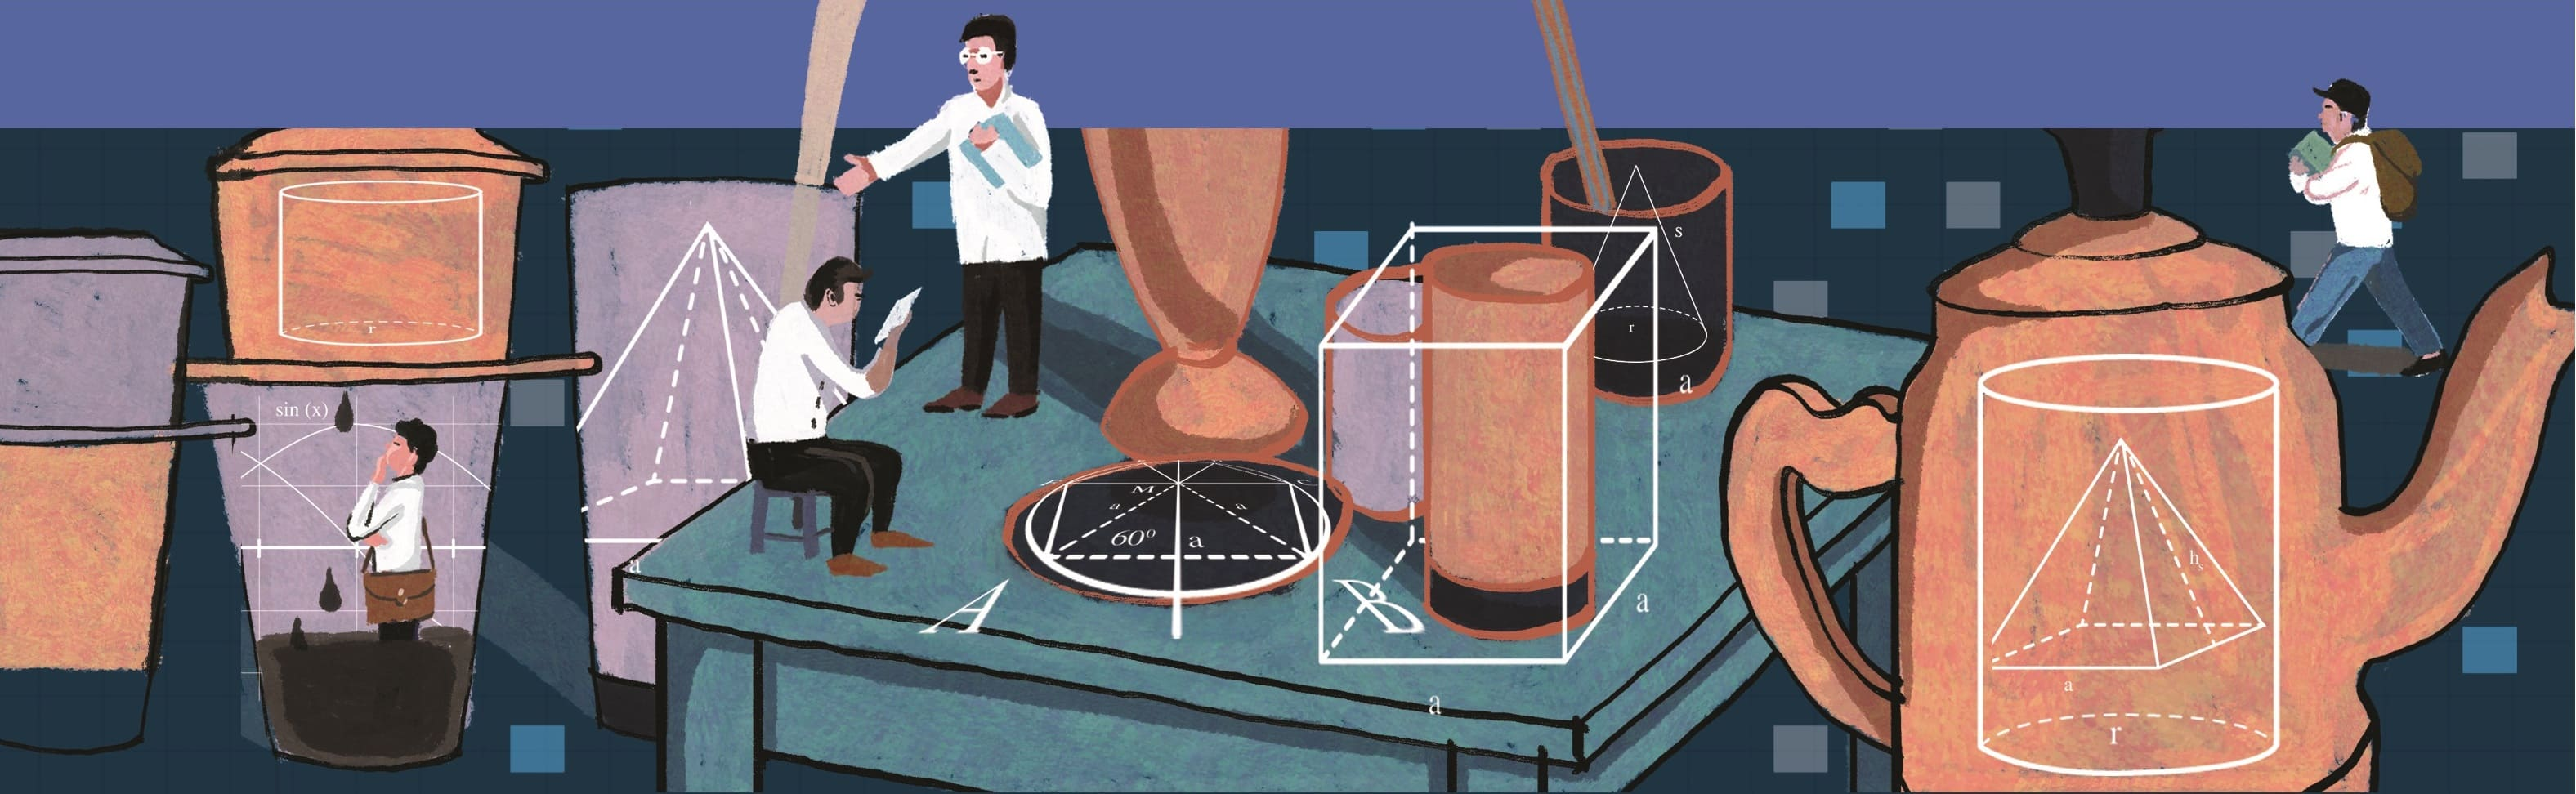
\includegraphics[width=19.3cm]{../bannerquantoan}}}
\AddToShipoutPicture*{\put(110,520){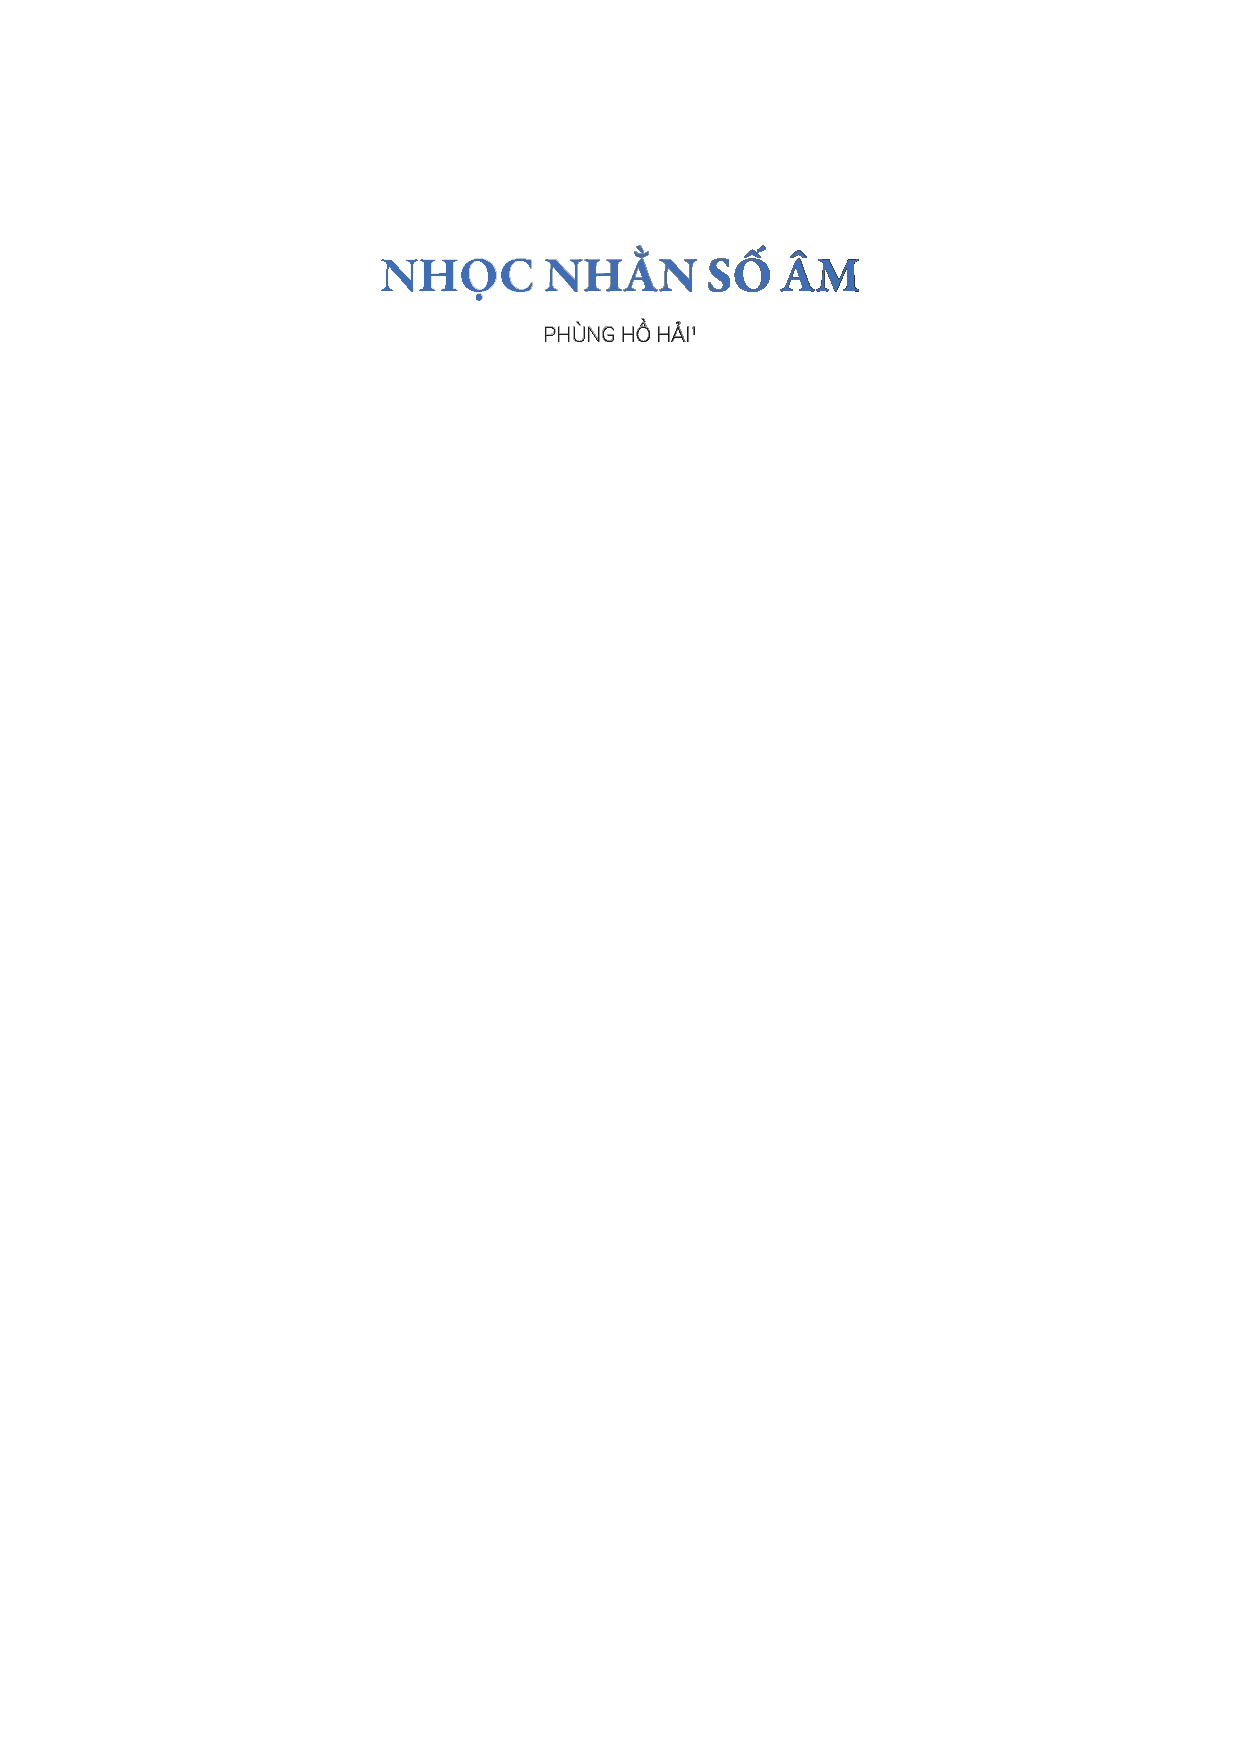
\includegraphics[scale=1]{../tieude3.pdf}}}
\centering
\endgroup

\vspace*{195pt}

\begin{multicols}{2}	
	\textbf{\color{quantoan}Dấu hiệu chia hết cho $\pmb{7}$ của Chika}
	\vskip 0.1cm
	Nhiều bạn đọc của Pi chắc đã quen thuộc với các dấu hiệu chia hết cho $2, 3, 5, 9, 11$, thường được học ở cuối bậc tiểu học hay ở những năm đầu của bậc trung học cơ sở. Chẳng hạn, một số tự nhiên chia hết cho $2$ khi và chỉ khi nó tận cùng là $0, 2, 4, 6$ hoặc $8$. Mặt khác, một số tự nhiên chia hết cho $3$ khi và chỉ khi tổng các chữ số của nó chia hết cho $3$. Ví dụ, số $2021$ có tổng các chữ số bằng $2+0+2+1=5$ không chia hết cho $3$ nên cũng không chia hết cho $3$. Những bạn đọc với bộ óc tò mò chắc hẳn đã từng đặt câu hỏi: \emph{Có dấu hiệu nào để nhận biết một số tự nhiên chia hết cho $7$ hay không?} 
	\vskip 0.1cm
	Hai năm trước, một cậu bé $12$ tuổi người Nigeria tên là Chika Ofili, theo học tại trường Westminster Underschool, Luân Đôn, Vương quốc Anh đã tình cờ tìm ra một câu trả lời đơn giản cho câu hỏi trên. Nói về  khám phá đầy bất ngờ đó, Mary Ellis, cô giáo của cậu, kể lại: 
	\vskip 0.1cm
	\emph{Tôi đưa cho cậu ấy một cuốn sách có tên ``Những bước đầu tiên cho người giải toán" để đọc trong dịp nghỉ hè và bên trong cuốn sách có liệt kê một số các phép thử, sử dụng để \linebreak nhanh chóng tìm ra liệu một số có chia hết cho $2, 3, 4, 5, 6, 8$ hoặc $9$ hay không, trước khi bạn thực sự bắt đầu thực hiện phép chia. Thế nhưng, trong cuốn sách không có phép thử nào để kiểm tra tính chia hết cho $7$. Lý do vì sao nó bị thiếu là không có phép thử nào dễ hoặc có thể ghi nhớ cho phép chia cho $7$, tôi nghĩ vậy!}
	\vskip 0.1cm
	\emph{Trong một khoảnh khắc buồn tẻ, Chika đã suy nghĩ về vấn đề này và đây là điều mà cậu ấy đã nghĩ ra. Cậu ấy nhận ra rằng nếu bạn lấy chữ số cuối cùng của bất kỳ số tự nhiên nào, nhân nó với $5$ và sau đó cộng nó với phần còn lại của số ban đầu, bạn sẽ được một số mới. Và hóa ra là nếu số mới chia hết cho $7$, thì số ban đầu chia hết cho $7$. Thật là một phép thử dễ dàng!}
	\vskip 0.1cm
	Và cô bổ sung thêm: ``\emph{Điều ngược lại cũng đúng: nếu số mới không chia hết cho $7$ thì số ban đầu cũng không chia hết cho $7$.}
	\vskip 0.1cm
	Chẳng hạn, ta hãy kiểm tra xem số $532$ có chia hết cho $7$ hay không bằng phép thử Chika:
	\vskip 0.1cm
	$\bullet$ $532 \rightsquigarrow 53+ 5 \times 2=63$.
	\vskip 0.1cm
	$\bullet$ $63$ chia hết cho $7$. Vậy $532$ chia hết cho $7$.
	\vskip 0.1cm
	Ta hãy lấy một ví dụ khác, chẳng hạn $4836$.
	\vskip 0.1cm
	$\bullet$ $4836 \rightsquigarrow 483+ 5 \times 6=483 + 30= 513$;
	\vskip 0.1cm
	$\bullet$ $513 \rightsquigarrow  51 + 5 \times 3= 66$;
	\vskip 0.1cm
	$\bullet$ $66$ không chia hết cho $7$. Vậy số $4836$ không chia hết cho $7$.
	\vskip 0.1cm
	Với phát hiện của mình, Chika Ofili đã vinh\linebreak dự nhận được giải thưởng \emph{Người hùng nhỏ bé đích thực} năm $2019$ (TruLittle Hero Awards). Đây là một một giải thưởng thường niên dành cho những học sinh dưới $17$ tuổi có những thành tích xuất sắc trên các lĩnh vực khác nhau của Vương quốc Anh. Một phần thưởng thật tuyệt vời!
	\begin{figure}[H]
		\vspace*{-5pt}
		\centering
		\captionsetup{labelformat= empty, justification=centering}
		\includegraphics[width= 0.475\textwidth]{chika}
		\caption{\small\textit{\color{quantoan}Chika nhận giải thưởng Người hùng nhỏ bé đích thực $2019$.}}
		\vspace*{-10pt}
	\end{figure}
	\textbf{\color{quantoan}Một số dấu hiệu chia hết cho $\pmb{7}$ khác}
	\vskip 0.1cm
	Cho dù không phổ biến bằng các dấu hiệu chia hết cho $2, 3, 4, 5, 8, 9$, nhiều dấu hiệu chia hết cho $7$ đã được các nhà toán học đưa ra. Sau đây là một vài tiêu chuẩn được trích từ [$1$].
	\vskip 0.1cm
	$1.$ Trong \emph{Talmud}, một bộ sách thánh của Do Thái giáo (khoảng thế kỷ thứ $5$ sau Công Nguyên), dấu hiệu sau đây được đề cập đến:  số tự nhiên $\overline{a_ka_{k-1}\ldots a_2 a_1 a_0}$ chia hết cho $7$ nếu và chỉ nếu $2\times  \overline{a_ka_{k-1}\ldots a_2} + \overline{a_1a_0}$ chia hết cho $7$. Nghĩa là, một số chia hết cho $7$ nếu và chỉ nếu lấy \emph{hai chữ số tận cùng cộng với hai lần số còn lại (khi bỏ hai chữ số tận cùng) thì được một số chia hết cho $7$.}
	\vskip 0.1cm
	Ví dụ, để kiểm tra số $483595$ có chia hết cho $7$ hay không, ta tiến hành các phép tính:
	\vskip 0.1cm
	$\bullet$ $483595 \rightsquigarrow	2\times 4835 + 95= 9765$;
	\vskip 0.1cm
	$\bullet$ $9765 \rightsquigarrow	2\times 97 + 65= 259$;
	\vskip 0.1cm
	$\bullet$ $259 \rightsquigarrow 2\times 2 + 59= 63$;
	\vskip 0.1cm
	$\bullet$ $63$ chia hết cho $7$. Vậy $483595$ chia hết \linebreak cho $7$.
	\vskip 0.1cm
	$2.$ Fibonacci, trong cuốn \emph{Liber Abaci}, xuất bản năm $1202$, phát biểu dấu hiệu sau đây: số tự nhiên $\overline{a_ka_{k-1}\ldots a_2 a_1 a_0}$ có cùng số dư với $a_0+3a_1+ 2a_2 -a_3 -3a_4 -2a_5 + a_6 + \cdots$ khi chia cho $7$. Nói riêng, $\overline{a_ka_{k-1}\ldots a_2 a_1 a_0}$ chia hết cho $7$ nếu và chỉ nếu $a_0+3a_1+ 2a_2 -a_3 -3a_4 -2a_5 + a_6 + \cdots$ chia hết cho $7$. Nghĩa là, một số chia hết cho $7$ nếu và chỉ nếu, khi lấy các chữ số của nó từ phải sang trái, nhân lần lượt với $(1, 3, 2, -1, -3, -2, \ldots)$ rồi cộng lại thì được một số chia hết cho $7$.
	\vskip 0.1cm
	Ta hãy áp dụng dấu hiệu của Fibonacci cho ví dụ trên đây:
	\vskip 0.1cm	
	$\bullet$ $483595 \rightsquigarrow	5+ 3\times 9 + 2\times 5 -3 -3\times 8 - 2\times 4=7$;
	\vskip 0.1cm
	$\bullet$ $7$ chia hết cho $7$. Vậy $483595$ chia hết cho~$7$.
	\vskip 0.1cm
	$3.$ (Dấu hiệu tổng đan dấu các khối $3$ chữ số liên tiếp.) Một số chia hết cho $7$ nếu tổng đan dấu của các khối ba chữ số, tính từ phải sang trái, chia hết cho $7$. Nói cách khác, một số tự nhiên $\overline{a_ka_{k-1}\ldots a_2 a_1 a_0}$ chia hết cho $7$ khi và chỉ khi tổng $\overline{a_2a_1a_0}- \overline{a_5a_4a_3}+ \cdots$ chia hết cho $7$. Một dạng tổng quát của dấu hiệu này được nhà toán học người Đức A.L Crelle đưa ra vào năm $1848$.
	\vskip 0.1cm
	Ví dụ, với số $8369851$ ta có:
	\vskip 0.1cm	
	$\bullet$ $8369851 \rightsquigarrow 851-369 + 8 = 490$;
	\vskip 0.1cm
	$\bullet$ $490 = 7 \times 70$  chia hết cho $7$. Vậy $8369851$ chia hết cho $7$.
	\vskip 0.1cm
	Vậy, dấu hiệu mà cậu bé Chika khám phá ra mới như thế nào? Rất tiếc, dấu hiệu mà cậu tìm ra có lẽ đã được biết đến từ trước. Chẳng hạn, vẫn theo [$1$], nó tương tự như dấu hiệu mà Zbikowski đưa ra vào năm $1861$:
	\vskip 0.1cm
	$4.$ Số tự nhiên $\overline{a_k a_{k-1}\ldots a_2a_1a_0}$ chia hết cho $7$ khi và chỉ khi $\overline{a_k a_{k-1}\ldots a_2a_1} -2a_0$ chia hết cho $7$.
	\vskip 0.1cm
	Mặc dầu vậy, việc phát hiện của Chika, một cậu học trò $12$ tuổi, đến từ những tìm tòi của riêng mình là một điều rất đỗi phi thường và đáng nể.
	\vskip 0.1cm
	\textbf{\color{quantoan}Một vài bài tập cho bạn đọc}
	\vskip 0.1cm
	Để kết thúc, tác giả xin mời các độc giả thử sức mình với một số bài toán nhỏ sau đây.
	\vskip 0.1cm
	$1.$ Kiểm tra xem các số sau đây có chia hết cho $7$ hay không: 
	\vskip 0.1cm
	$(a)$ $2945$;
	\vskip 0.1cm
	$(b)$ $271828$;
	\vskip 0.1cm
	$(c)$ $314159$;
	\vskip 0.1cm
	dựa vào các dấu hiệu Chika, Talmud, \linebreak Fibonacci và dấu hiệu tổng đan dấu các khối ba chữ số.
	\vskip 0.1cm	
	$2.$ (Dấu hiệu chia hết cho $7$ của Chika.)\linebreak Chứng minh rằng số tự nhiên \linebreak $ \overline{a_k a_{k-1}\ldots a_2a_1a_0}$ chia hết cho $7$ khi và chỉ khi  $ \overline{a_k a_{k-1}\ldots a_2a_1} +5\times a_0$ chia hết cho $7$.
	\vskip 0.1cm	
	$3.$ (Dấu hiệu chia hết cho $7$ của Fibonacci.)\linebreak Chứng minh rằng mọi số tự nhiên $\overline{a_k a_{k-1}\ldots a_1a_0}$ có cùng số dư với $a_0+3a_1+ 2a_2 -a_3 -3a_4 -2a_5 + a_6 + \cdots$ khi chia \linebreak cho $7$.
	\vskip 0.1cm	
	$4.$ (Dấu hiệu chia hết cho $7$ trong Talmud.)\linebreak Chứng minh rằng mọi số tự nhiên $\overline{a_k a_{k-1}\ldots a_1a_0}$ có cùng số dư với $2\overline{a_k a_{k-1}\ldots a_2} + \overline{a_1a_0}$ khi chia cho $7$. 
	\vskip 0.1cm
	\textbf{\color{quantoan}Tài liệu}
	\vskip 0.1cm	
	[$1$] Dickson, L. E. \textit{History of the theory of numbers}, Vol.$1$, $1919$.
	\vskip 0.1cm 
	[$2$] Trang wikipedia \textit{https://en.wikipedia.org/\\wiki/Divisibility\_rule}.
	\vskip 0.1cm
	[$3$] Trang \textit{https://www.westminsterunder.org.\\uk/chikas-test/}.
\end{multicols}
%\vspace*{-10pt}
%\rule{1\textwidth}{0.1pt}
%\begin{center}
%	\textbf{\LARGE\color{quantoan}LỜI GIẢI, ĐÁP ÁN}
%\end{center}
%\begin{multicols}{2}
%	\textbf{\color{quantoan}Đố vui} 
%	\vskip 0.1cm
%	Trả lời: Tất cả đều là người nói dối!
%	\vskip 0.1cm
%	Giả sử có một người nói thật, ký hiệu là $A_1$. Như vậy, anh ta ngồi bên cạnh một người nói dối và một người nói thật: chẳng hạn bên trái của $A_1$ là một người nói dối, ký hiệu là $A_0$ và bên phải của anh ta là một người nói thật, ký hiệu là $A_2$. Do $A_2$ nói thật (và $A_1$  cũng là người nói thật) nên người ngồi bên phải của anh ta, ký hiệu là $A_3$, là người nói dối. Do $A_3$ là người nói dối (và $A_2$ nói thật) nên người ngồi bên phải của anh ta, ký hiệu là $A_4$, không thể là người nói dối mà phải là một người nói thật. Từ đó, với cách lập luận như trên, ta thấy rằng số các người trên bàn phải chia hết cho $3$ (vì sẽ lặp lại mẫu Thật--Thật--Dối--Thật--Thật--Dối \ldots). Mà $10$ không chia hết cho $3$ nên ta có điều vô lý.
%	\vskip 0.1cm
%	\textbf{\color{quantoan}Trùm trộm sa lưới}
%	\vskip 0.1cm
%	$a$) Các em thấy ngay trong ngày thứ Tư chỉ có Phong và Linh tại cửa hàng. Vì Phong đã có ở đó hôm thứ Hai, nên thứ Ba phải có \linebreak Linh và Kính trực. Lập luận tiếp tục như vậy ta có thể điền lịch trực theo dõi của $3$ người trong $6$ ngày liên tiếp đó như Bảng $1$.
%	\vskip 0.1cm
%	$b)$ Các em có thể thấy ngay, theo ngược chiều kim đồng hồ, các nhân vật lần lượt là Sinh, Lệ, Kính, Phong (do Cường và Linh ngồi cạnh nhau, nên không thể ngồi giữa Lệ và Phong). Tiếp theo đó là Bùi Linh và tên Cường bự.
%\end{multicols}
%\begin{table}[H]
%	\setlength{\tabcolsep}{15pt}
%	\renewcommand{\arraystretch}{1.3}
%	\vspace*{-5pt}
%	\centering
%	\captionsetup{labelformat= empty, justification=centering}
%	\begin{tabular}{|c|c|c|c|c|c|}
%		\hline
%		Thứ Hai&	Thứ Ba&	Thứ Tư&	Thứ Năm&	Thứ Sáu&	Thứ Bảy\\
%		\hline
%		Phong& Linh& Phong &Phong &Linh & Phong\\
%		\hline
%		Kính&Kính&Linh&Kính&Kính&Linh\\
%		\hline
%	\end{tabular}
%	\caption{\small\textit{\color{quantoan}Bảng $1$.}}
%	\vspace*{-10pt}
%\end{table}